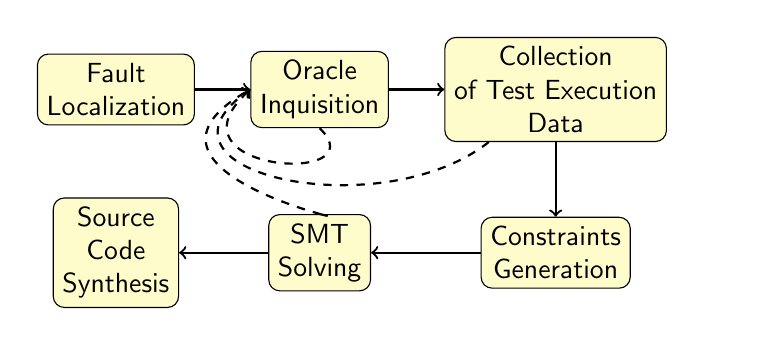
\begin{tikzpicture}[
  font=\sffamily,
  every matrix/.style={ampersand replacement=\&,column sep=2em,row sep=2em},
  box/.style={draw,rounded corners,fill=yellow!20},
  flow/.style={->, thick},
  fail/.style={->, thick, dashed},
  every node/.style={align=center}]
  
% Position the nodes using a matrix layout
\matrix{
    \node[box] (faultLocalization) {Fault \\ Localization};
      \& \node[box] (oracleInquisition) {Oracle \\ Inquisition};
      \& \node[box] (collectionOfTestExecutionData) {Collection \\ of Test Execution \\ Data};
      \& \\

    \node[box] (sourceCodeSynthesis) {Source \\ Code \\ Synthesis};
      \& \node[box] (smtSolving) {SMT \\ Solving};
      \& \node[box] (constraintsGeneration) {Constraints \\ Generation}; \\
  };

% Draw the arrows between the nodes and label them.
\draw [flow] (faultLocalization) -- (oracleInquisition);
\draw [flow] (oracleInquisition) -- (collectionOfTestExecutionData);
\draw [flow] (collectionOfTestExecutionData) -- (constraintsGeneration);
\draw [flow] (constraintsGeneration) -- (smtSolving);
\draw [flow] (smtSolving) -- (sourceCodeSynthesis);

\draw [fail] (oracleInquisition.south) .. controls (down:.5em) and (left:8em) .. (oracleInquisition.west);
\draw [fail] (collectionOfTestExecutionData) .. controls (down:2em) and (left:9em) .. (oracleInquisition.west);
\draw [fail] (smtSolving.north) .. controls (down:2em) and (left:10em) .. (oracleInquisition.west);
\end{tikzpicture}
